\section{Discussion}

\subsection{Forces et faiblesses du modèle}
Dans ce projet de recherche, j'ai réussi à développer un algorithme de rendu pouvant représenter les cheveux comme un GPIS. Cet accomplissement permet de confirmer que les cheveux peuvent s'insérer harmonieusement dans le continuum présenté par \textcite{seyb24from}, ce qui représente un pas prometteur pour l'utilisation de GPIS pour tous les éléments d'une scène.

De plus, l'utilisation d'un format d'encodage des cheveux déjà utilisé permet de démocratiser l'approche GPIS. En effet, puisque cette technique est nouvelle, il n'y a pas d'outils pour artistes permettant le développement de dessins 3D rendus vers le GPIS ; ainsi, en ayant un encodage populaire, on facilite l'export de modèles vers un moteur de rendu GPIS. Il permet aussi une comparaison très facile avec le rendu des mêmes cheveux avec une technique de tracé de rayon traditionnel.

Une faiblesse de mon modèle est l'utilisation d'une moyenne par SDF. En effet, si on cherche à rendre l'algorithme de rendu différentiable (un des gros avantages des GPIS), l'approximation en capsule de la courbe du cheveu est déjà différentiable sans l'ajout de la couche GPIS avec une variance. En effet, contrairement aux géométries maillées, les fonctions de distance signée sont déjà facilement différentiables et utilisées pour faire du rendu différentiable \cite{vicini2022sdf}. Toutefois, il est intéressant de mentionner que la couche GPIS conserve la différentiabilité de la SDF et donne ainsi accès au continuum volume/solide, ce qui permet de jouer avec l'apparence du rendu du cheveu.

Une autre faiblesse est l'aspect micro de l'effet stochastique. En effet, puisque les cheveux sont très petits, il n'est pas possible d'obtenir l'effet de rugosité comme dans les rendus à plus large échelle de \textcite{xu25practical}. Le résultat obtenu est plutôt binaire : les cheveux sont soit détectés à l'endroit espéré, soit transformés en fils trop minces pour être rendus.

\begin{figure}[H]
    \centering
    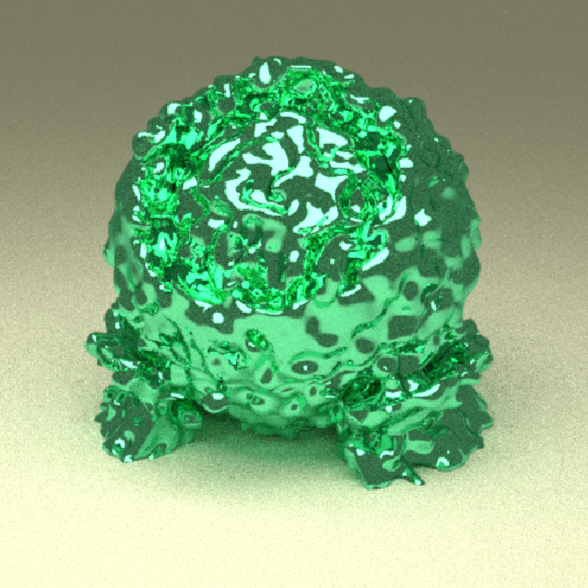
\includegraphics[width=0.7\textwidth]{figures/shadertoy_exmaple_rugeux.png}
    \caption{Un exemple de la démo de \textcite{xu25practical} démontrant la rugosité de la surface à une échelle visible.}
    \label{fig:shadertoy_rugueux}
\end{figure}

Le programme de rendu développé dans ce projet \cite{felixg13gpis} a subi plusieurs itérations. Initialement, j'ai tenté d'utiliser le moteur de rendu Mitsuba 3 \cite{Mitsuba3}, qui est un moteur de rendu différentiable et axé sur la recherche. Il expose une interface de \texttt{plugin} Python qui semblait idéale pour le développement d'un nouveau type d'élément de scène. Après une longue phase de découverte, j'ai compris que l'interface Python ne permet pas l'ajout d'une nouvelle sorte de volume ; il fallait donc créer une duplication (fork) du projet et modifier le code C++ directement. Malheureusement, cette approche est trop mal documentée et le progrès n'était pas assez rapide pour un projet de recherche. Il serait toutefois très intéressant de faire l'implémentation des GPIS dans le moteur de rendu Mitsuba 3, ce qui serait une étape importante pour la démocratisation de cette technique. Cela représente un projet de recherche complet à lui seul. 

L'itération suivante a donc été de faire une implémentation complète d'un moteur de rendu en Python ; avoir le contrôle complet sur le moteur devrait assurer d'avoir le strict nécessaire pour évaluer la technique, ce qui permettrait des itérations plus rapides. Pour assurer la performance du moteur, Numba \cite{lam2015numba} avait été retenu comme solution pour précompiler le Python vers du langage machine et ainsi pallier la non-performance de l'interpréteur Python. Des problèmes de performance sont toutefois survenus lors de l'algorithme de traversée de la hiérarchie de volumes englobants pour des millions de cheveux ; en effet, cette traversée est faite à répétition et doit être très performante. Développer cette optimisation serait en elle-même aussi un projet de recherche complet. En fait, des solutions matérielles comme les circuits logiques dédiés sur les GPU modernes \cite{nvidia_rtx} ou l'algorithmique avancée d'Embree \cite{wald2014embree} ont déjà résolu ce problème de performance.

C'est pourquoi la dernière itération du programme de ce projet de recherche a été de créer un moteur de rendu par tracé de rayon basé sur Embree. Cela m'a permis d'obtenir des performances intéressantes compte tenu de la complexité temporelle de l'algorithme étudié. Le code pourrait être raffiné en utilisant des opérations SIMD pour échantillonner le GPIS sur plusieurs points le long du rayon en même temps. Une itération future encore plus performante serait une implémentation sur carte graphique à l'aide d'OpenGL et GLSL ; d'ailleurs, \textcite{xu25practical} présente une démo de leur implémentation sur ShaderToy en GLSL \cite{xu2025shadertoy}.
